%%%%%%%%%%%%%%%%%%%%%%%%%%%%%%%%%%%%%%%%%%%%%%%%%
% Chapter: Introduction
%%%%%%%%%%%%%%%%%%%%%%%%%%%%%%%%%%%%%%%%%%%%%%%%%
\chapter{Introduction}
\label{chap:intro}

The \ac{PMI} has been used for quite some time as a means of exchanging wireup information needed for inter-process communication.
Two versions (PMI-1 and PMI-2) have been released as part of the MPICH effort, with PMI-2 demonstrating better scaling properties than its PMI-1 predecessor. However, two significant challenges face the \ac{HPC} community as it continues to move towards machines capable of exaflop and higher performance levels:

\begin{itemize}
\item the physical scale of the machines, and the corresponding number of total processes they support, is expected to reach levels approaching  1 million processes executing across 100 thousand nodes. Prior methods for initiating applications relied on exchanging communication endpoint information between the processes, either directly or in some form of hierarchical collective operation. Regardless of the specific mechanism employed, the exchange across such large applications would consume considerable time, with estimates running in excess of 5-10 minutes; and
\item whether it be hybrid applications that combine OpenMP threading operations with MPI, or application-steered workflow computations, the HPC community is experiencing an unprecedented wave of new approaches for computing at exascale levels. One common thread across the proposed methods is an increasing need for orchestration between the application and the \ac{SMS} comprising the scheduler (a.k.a. the \ac{WLM}), the \ac{RM}, global file system, fabric, and other subsystems. The lack of available support for application-to-SMS integration has forced researchers to develop "virtual" environments that hide the SMS behind a customized abstraction layer, but this results in considerable duplication of effort and a lack of portability.
\end{itemize}

\ac{PMIx} represents an attempt to resolve these questions by providing an extended version of the \ac{PMI} definitions specifically designed to support clusters up to exascale and larger sizes.
The overall objective of the project is not to branch the existing definitions -- in fact, \ac{PMIx} fully supports both of the existing PMI-1 and PMI-2 \acp{API} -- but rather to:

\begin{compactalphaenum}
\item add flexibility to the existing \acp{API} by adding an array of key-value ``attribute'' pairs to each \ac{API} signature that allows implementers to customize the behavior of the \ac{API} as future needs emerge without having to alter or create new variants of it;

\item add new APIs that provide extended capabilities such as asynchronous event notification plus dynamic resource allocation and management;

\item establish a collaboration between \ac{SMS} subsystem providers including resource manager, fabric, file system, and programming library developers to define integration points between the various subsystems as well as agreed upon definitions for associated \acp{API}, attribute names, and data types;

\item form a standards-like body for the definitions; and

\item provide a reference implementation of the \ac{PMIx} standard.
\end{compactalphaenum}

Complete information about the \ac{PMIx} standard and affiliated projects can be found at the \ac{PMIx} web site: \url{https://pmix.org}


%%%%%%%%%%%%%%%%%%%%%%%%%%%%%%%%%%%%%%%%%%%%%%%%%
%%%%%%%%%%%%%%%%%%%%%%%%%%%%%%%%%%%%%%%%%%%%%%%%%
\section{Charter}
\label{chap:intro:charter}

The charter of the PMIx community is to:
\begin{itemize}
\item Define a set of agnostic APIs (not affiliated with any specific programming model or code base) to support interactions between application processes and the \ac{SMS}.
\item Develop an open source (non-copy-left licensed) standalone ``reference'' library implementation to facilitate adoption of the \ac{PMIx} standard.
\item Retain transparent backward compatibility with the existing PMI-1 and PMI-2 definitions, any future \ac{PMI} releases, and across all \ac{PMIx} versions.
\item Support the ``Instant On'' initiative for rapid startup of applications at exascale and beyond.
\item Work with the \ac{HPC} community to define and implement new \acp{API} that support evolving programming model requirements for application interactions with the \ac{SMS}.
\end{itemize}

Participation in the \ac{PMIx} community is open to anyone, and not restricted to only code contributors to the reference implementation.


%%%%%%%%%%%%%%%%%%%%%%%%%%%%%%%%%%%%%%%%%%%%%%%%%
%%%%%%%%%%%%%%%%%%%%%%%%%%%%%%%%%%%%%%%%%%%%%%%%%
\section{PMIx Standard Overview}
\label{chap:intro:std_overview}

The \ac{PMIx} Standard defines and describes the interface developed by the \acf{PRI}.
Much of this document is specific to the \acf{PRI}'s design and implementation.
Specifically the standard describes the functionality provided by the \ac{PRI}, and what the \ac{PRI} requires of the clients and \acfp{RM} that use it's interface.

%%%%%%%%%%%
\subsection{Who should use the standard?}

The \ac{PMIx} Standard informs PMIx clients and \acp{RM} of the syntax and semantics of the \ac{PMIx} APIs.

\ac{PMIx} clients (e.g., tools, \ac{MPE} libraries) can use this standard to understand the set of attributes provided by various APIs of the \ac{PRI} and their intended behavior.
Additional information about the rationale for the selection of specific interfaces and attributes is also provided.

\ac{PMIx}-enabled \acp{RM} can use this standard to understand the expected behavior required of them when they support various interfaces/attributes.
In addition, optional features and suggestions on behavior are also included in the discussion to help guide \ac{RM} design and implementation.

%%%%%%%%%%%
\subsection{What is defined in the standard?}

The \ac{PMIx} Standard defines and describes the interface developed by the \acf{PRI}.
It defines the set of attributes that the \ac{PRI} supports; the set of attributes that are required of a \ac{RM} to support, for a given interface; and the set of optional attributes that an \ac{RM} may choose to support, for a given interface.

%%%%%%%%%%%
\subsection{What is \emph{not} defined in the standard?}

No standards body can require an implementer to support something in their standard, and \ac{PMIx} is no different in that regard. While an implementer of the \ac{PMIx} library itself must at least include the standard \ac{PMIx} headers and instantiate each function, they are free to return ``not supported'' for any function they choose not to implement.

This also applies to the host environments. Resource managers and other system management stack components retain the right to decide on support of a particular function. The \ac{PMIx} community continues to look at ways to assist \ac{SMS} implementers in their decisions by highlighting functions that are critical to basic application execution (e.g., \refapi{PMIx_Get}), while leaving flexibility for tailoring a vendor's software for their target market segment.

One area where this can become more complicated is regarding the attributes that provide information to the client process and/or control the behavior of a \ac{PMIx} standard \ac{API}. For example, the \refattr{PMIX_TIMEOUT} attribute can be used to specify the time (in seconds) before the requested operation should time out. The intent of this attribute is to allow the client to avoid ``hanging'' in a request that takes longer than the client wishes to wait, or may never return (e.g., a \refapi{PMIx_Fence} that a blocked participant never enters).

If an application (for example) truly relies on the \refattr{PMIX_TIMEOUT} attribute in a call to \refapi{PMIx_Fence}, it should set the required flag in the \refstruct{pmix_info_t} for that attribute. This informs the library and its \ac{SMS} host that it must return an immediate error if this attribute is not supported. By not setting the flag, the library and \ac{SMS} host are allowed to treat the attribute as optional, ignoring it if support is not available.

It is therefore critical that users and application implementers:

\begin{compactalphaenum}
\item consider whether or not a given attribute is required, marking it accordingly; and

\item check the return status on all \ac{PMIx} function calls to ensure support was present and that the request was accepted. Note that for non-blocking \acp{API}, a return of \refconst{PMIX_SUCCESS} only indicates that the request had no obvious errors and is being processed – the eventual callback will return the status of the requested operation itself.
\end{compactalphaenum}

While a \ac{PMIx} library implementer, or an \ac{SMS} component server, may choose to support a particular \ac{PMIx} \ac{API}, they are not required to support every attribute that might apply to it. This would pose a significant barrier to entry for an implementer as there can be a broad range of applicable attributes to a given \ac{API}, at least some of which may rarely be used. The \ac{PMIx} community is attempting to help differentiate the attributes by indicating those that are generally used (and therefore, of higher importance to support) vs those that a ``complete implementation'' would support.

Note that an environment that does not include support for a particular attribute/\ac{API} pair is not ``incomplete'' or of lower quality than one that does include that support. Vendors must decide where to invest their time based on the needs of their target markets, and it is perfectly reasonable for them to perform cost/benefit decisions when considering what functions and attributes to support.

The flip side of that statement is also true: Users who find that their current vendor does not support a function or attribute they require may raise that concern with their vendor and request that the implementation be expanded. Alternatively, users may wish to utilize the \ac{PRRTE} as a ``shim'' between their application and the host environment as it might provide the desired support until the vendor can respond. Finally, in the extreme, one can exploit the portability of PMIx-based applications to change vendors.

%%%%%%%%%%%
\subsection{General Guidance for PMIx Users and Implementors}

The \ac{PMIx} Standard defines the behavior of the \acf{PRI}.
A complete system harnessing the \ac{PMIx} interface requires an agreement between the \ac{PMIx} client, be it a tool or library, and the \ac{PMIx}-enabled \ac{RM}.
The \ac{PRI} acts as an intermediary between these two entities by providing a standard API for the exchange of requests and responses.
The degree to which the \ac{PMIx} client and the \ac{PMIx}-enabled \ac{RM} may interact needs to be defined by those developer communities.
The \ac{PMIx} standard can be used to define the specifics of this interaction.

\ac{PMIx} clients (e.g., tools, \ac{MPE} libraries) may find that they depend only on a small subset of interfaces and attributes to work correctly.
\ac{PMIx} clients are strongly advised to define a document itemizing the \ac{PMIx} interfaces and associated attributes that are required for correct operation, and are optional but recommended for full functionality.
The \ac{PMIx} standard cannot define this list for all given \ac{PMIx} clients, but such a list is valuable to \acp{RM} desiring to support these clients.

\ac{PMIx}-enabled \acp{RM} may choose to implement a subset of the \ac{PMIx} standard and/or define attributes beyond those defined herein.
\ac{PMIx}-enabled \acp{RM} are strongly advised to define a document itemizing the \ac{PMIx} interfaces and associated attributes they support, with any annotations about behavior limitations.
The \ac{PMIx} standard cannot define this list for all given \ac{PMIx}-enabled \acp{RM}, but such a list is valuable to \ac{PMIx} clients desiring to support a broad range of \ac{PMIx}-enabled \acp{RM}.



%%%%%%%%%%%%%%%%%%%%%%%%%%%%%%%%%%%%%%%%%%%%%%%%%
%%%%%%%%%%%%%%%%%%%%%%%%%%%%%%%%%%%%%%%%%%%%%%%%%
\section{PMIx Architecture Overview}
\label{chap:intro:arch_overview}

This section presents a brief overview of the \ac{PMIx} Architecture~\cite{2017-Castain-EuroMPI}.
Note that this is a conceptual model solely used to help guide the standards process --- it does not represent
a design requirement on any \ac{PMIx} implementation. Instead, the model is used by the
\ac{PMIx} community as a sounding board for evaluating proposed interfaces and avoid unintentionally imposing
constraints on implementers. Built into the model are two guiding principles also reflected in the standard. First,
\ac{PMIx} operates in the mode of a \textit{messenger}, and not a \textit{doer} --- i.e., the role
of \ac{PMIx} is to provide communication between the various participants, relaying requests and returning
responses. The intent of the standard is not to suggest that \ac{PMIx} itself actually perform any of
the defined operations --- this is left to the various \ac{SMS} elements and/or the application. Any exceptions to that intent are left to the discretion of the particular implementation.

\begingroup
\begin{figure*}[ht!]
  \begin{center}
    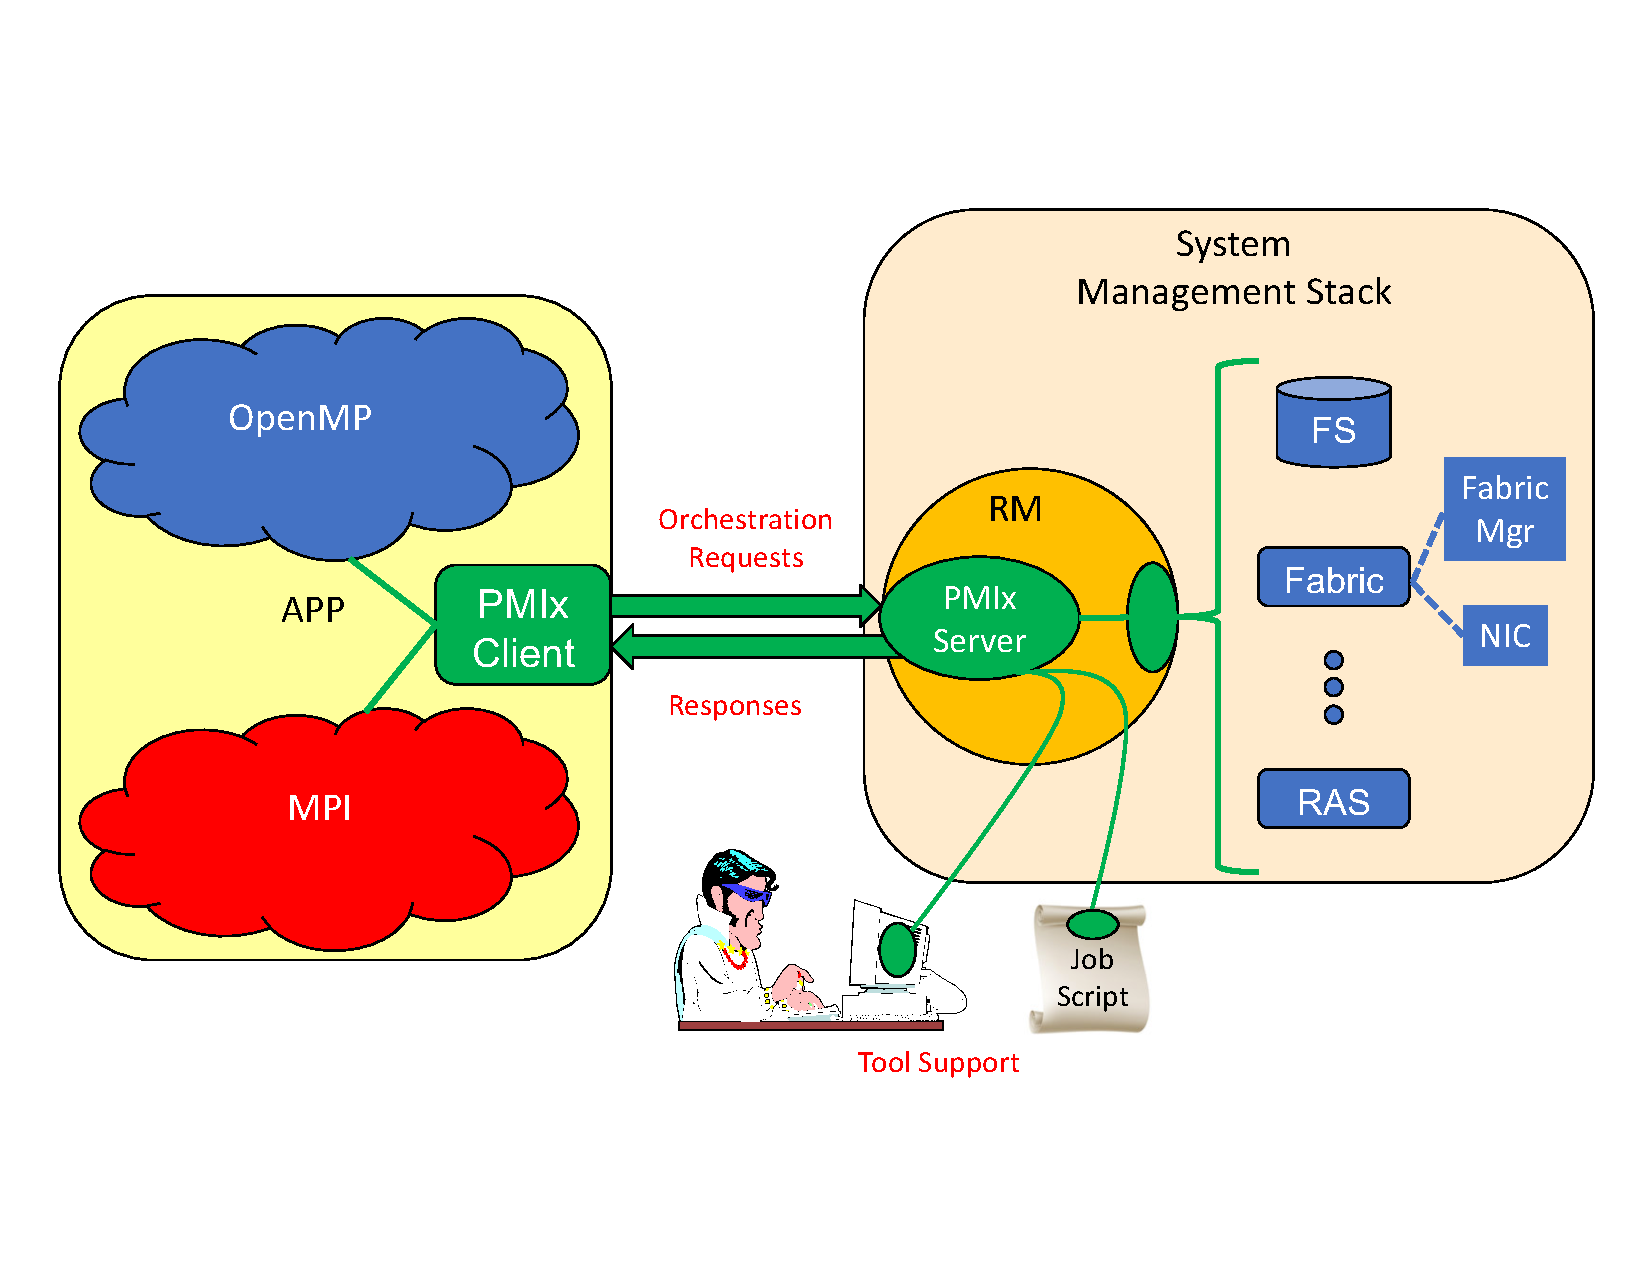
\includegraphics[clip,width=0.8\textwidth]{figs/PMIxRoles.pdf}
  \end{center}
  \caption{PMIx-SMS Interactions}
  \label{fig:roles}
\end{figure*}
\endgroup


Thus, as the diagram in Fig.~\ref{fig:roles} shows, the application is built against a \ac{PMIx} client library that contains the client-side \acp{API},
attribute definitions, and communication support for interacting with the local \ac{PMIx} server. Intra-process cross-library interactions
are supported at the client level to avoid unnecessary burdens on the server. Orchestration requests are sent to the
local \ac{PMIx} server, which subsequently passes them to the host \ac{SMS} (here represented by an \ac{RM} daemon) using the \ac{PMIx} server callback functions the host \ac{SMS} registered during PMIx\_server\_init. The host \ac{SMS} can indicate its lack of support for any operation by simply providing a \textit{NULL} for the associated callback function, or can create a function entry that returns \textit{not supported} when called.

The conceptual model places the burden of fulfilling the request on the host \ac{SMS}. This includes performing any
inter-node communications, or interacting with other \ac{SMS} elements. Thus, a client request for a network traffic report
does not go directly from the client to the \ac{FM}, but instead is relayed to the \ac{PMIx} server, and then passed to the host \ac{SMS}
for execution. This architecture reflects the second principle underlying the standard --- namely, that connectivity is to be minimized by channeling all application interactions with the \ac{SMS} through the local \ac{PMIx} server.

Recognizing the burden this places on SMS vendors, the PMIx community has included interfaces by
which the host can request support from local SMS elements. Once the SMS has transferred the request to
an appropriate location, a PMIx server interface can be used to pass the request between SMS subsystems.
For example, a request for network traffic statistics can utilize the
PMIx networking abstractions to retrieve the information from the FM. This reduces the portability and
interoperability issues between the individual subsystems by transferring the burden of defining the
interoperable interfaces from the SMS subsystems to the PMIx community, which continues
to work with those providers to develop the necessary support.

Tools, whether standalone or embedded in job scripts, are an exception to the communication rule and can connect to
any PMIx server providing they are given adequate rendezvous information. The PMIx conceptual model views the
collection of PMIx servers as a cloud-like conglomerate --- i.e., orchestration and information requests can be
given to any server regardless of location. However, tools frequently execute on locations that may not house an
operating PMIx server --- e.g., a users notebook computer. Thus, tools need the ability to remotely connect to
the PMIx server ``cloud''.

The scope of the PMIx standard therefore spans the range of these interactions, between client-and-SMS and between SMS
subsystems. Note again that this does not impose a requirement on any given PMIx implementation to cover the entire
range --- implementers are free to return \textit{not supported} from any PMIx function.


%%%%%%%%%%%
\subsection{The \acf{PRI}}

The \ac{PMIx} community has committed to providing a complete, reference implementation of each version of the standard. Note that the definition of the \ac{PMIx} Standard is not contingent upon use of the \acf{PRI} --- any implementation that supports the defined \acp{API} is a \ac{PMIx} Standard compliant implementation.
The \ac{PRI} is provided solely for the following purposes:
\begin{itemize}
\item Validation of the standard.\\
No proposed change and/or extension to the \ac{PMIx} standard is accepted without an accompanying prototype implementation in the \ac{PRI}.
This ensures that the proposal has undergone at least some minimal level of scrutiny and testing before being considered.
\item Ease of adoption.\\
The \ac{PRI} is designed to be particularly easy for resource managers (and the \ac{SMS} in general) to adopt, thus facilitating a rapid uptake into that community for application portability.
Both client and server \ac{PMIx} libraries are included, along with examples of client usage and server-side integration.
A list of supported environments and versions is maintained on the \ac{PMIx} web site \url{https://pmix.org/support/faq/what-apis-are-supported-on-my-rm/}
\end{itemize}

The \ac{PRI} does provide some internal implementations that lie outside the scope of the \ac{PMIx} standard. This includes several convenience macros as well as support for consolidating collectives for optimization purposes (e.g., the \ac{PMIx} server aggregates all local \refapi{PMIx_Fence} calls before
passing them to the \ac{SMS} for global execution). In a few additional cases, the \ac{PMIx} community (in partnership with the \ac{SMS} subsystem providers) have determined that a base level of support for a given operation can best be portably provided by including it in the \ac{PRI}.

Instructions for downloading, and installing the \ac{PRI} are available
on the community's web site \url{https://pmix.org/code/getting-the-reference-implementation/}.The \ac{PRI} targets support for the Linux operating system.
A reasonable effort is made to support all major, modern Linux distributions; however, validation is limited to the most recent 2-3 releases of RedHat Enterprise Linux (RHEL), Fedora, CentOS, and SUSE Linux Enterprise Server (SLES).
In addition, development support is maintained for Mac OSX.
Production support for vendor-specific operating systems is included as provided by the vendor.


%%%%%%%%%%%
\subsection{The PMIx Reference RunTime Environment (PRRTE)}

The \ac{PMIx} community has also released \ac{PRRTE} --- i.e., a runtime environment
containing the reference implementation and capable of operating within a host \ac{SMS}. \ac{PRRTE}
provides an easy way of exploring \ac{PMIx} capabilities and testing PMIx-based
applications outside of a PMIx-enabled environment by providing a ``shim'' between the application and the host environment that includes full support for the \ac{PRI}. The intent of \ac{PRRTE} is not to replace any existing production environment, but rather to enable developers to work on systems that do not yet feature a PMIx-enabled host \ac{SMS} or one that lacks a \ac{PMIx} feature of interest. Instructions for downloading,
installing, and using \ac{PRRTE} are available
on the community's web site \url{https://pmix.org/code/getting-the-pmix-reference-server/}

%%%%%%%%%%%%%%%%%%%%%%%%%%%%%%%%%%%%%%%%%%%%%%%%%
\section{Organization of this document}

The remainder of this document is structured as follows:

\begin{itemize}
\item Introduction and Overview in \chapterref{chap:intro}
\item Terms and Conventions in \chapterref{chap:terms}
\item Data Structures and Types in \chapterref{chap:struct}
\item \ac{PMIx} Initialization and Finalization in \chapterref{chap:api_init}
\item Key/Value Management in \chapterref{chap:api_kv_mgmt}
\item Process Management in \chapterref{chap:api_proc_mgmt}
\item Job Management in \chapterref{chap:api_job_mgmt}
\item Event Notification in \chapterref{chap:api_event}
\item Data Packing and Unpacking in \chapterref{chap:api_data_mgmt}
\item \ac{PMIx} Server Specific Interfaces in \chapterref{chap:api_server}
\end{itemize}

%%%%%%%%%%%%%%%%%%%%%%%%%%%%%%%%%%%%%%%%%%%%%%%%%
%%%%%%%%%% History: Version 1.0
\section{Version 1.0: June 12, 2015}

\par
The \ac{PMIx} version 1.0 \textit{ad hoc} standard was defined in the \acf{PRI} header files as part of the \ac{PRI} v1.0.0 release prior to the creation of the formal \ac{PMIx} 2.0 standard.
Below are a summary listing of the interfaces defined in the 1.0 headers.

\begin{itemize}
\item Client APIs
\begin{itemize}
\item PMIx\_Init, \refapi{PMIx_Initialized}, \refapi{PMIx_Abort}, \refapi{PMIx_Finalize}
\item \refapi{PMIx_Put}, \refapi{PMIx_Commit},
\item \refapi{PMIx_Fence}, \refapi{PMIx_Fence_nb}
\item \refapi{PMIx_Get}, \refapi{PMIx_Get_nb}
\item \refapi{PMIx_Publish}, \refapi{PMIx_Publish_nb}
\item \refapi{PMIx_Lookup}, \refapi{PMIx_Lookup}
\item \refapi{PMIx_Unpublish}, \refapi{PMIx_Unpublish_nb}
\item \refapi{PMIx_Spawn}, \refapi{PMIx_Spawn_nb}
\item \refapi{PMIx_Connect}, \refapi{PMIx_Connect_nb}
\item \refapi{PMIx_Disconnect}, \refapi{PMIx_Disconnect_nb}
\item \refapi{PMIx_Resolve_nodes}, \refapi{PMIx_Resolve_peers}
\end{itemize}
\item Server APIs
\begin{itemize}
\item \refapi{PMIx_server_init}, \refapi{PMIx_server_finalize}
\item \refapi{PMIx_generate_regex}, \refapi{PMIx_generate_ppn}
\item \refapi{PMIx_server_register_nspace}, \refapi{PMIx_server_deregister_nspace}
\item \refapi{PMIx_server_register_client}, \refapi{PMIx_server_deregister_client}
\item \refapi{PMIx_server_setup_fork}, \refapi{PMIx_server_dmodex_request}
\end{itemize}
\item Common APIs
\begin{itemize}
\item \refapi{PMIx_Get_version}, \refapi{PMIx_Store_internal}, \refapi{PMIx_Error_string}
\item \code{PMIx_Register_errhandler}, \code{PMIx_Deregister_errhandler}, \code{PMIx_Notify_error}
\end{itemize}
\end{itemize}

The \code{PMIx_Init} \ac{API} was subsequently modified in the \ac{PRI} release v1.1.0.

%%%%%%%%%%%%%%%%%%%%%%%%%%%%%%%%%%%%%%%%%%%%%%%%%
%%%%%%%%%% History: Version 2.0
\section{Version 2.0: Sept. 2018}

The following \acp{API} were introduced in v2.0 of the PMIx Standard:

\begin{itemize}
\item Client APIs
\begin{itemize}
\item \refapi{PMIx_Query_info_nb}, \refapi{PMIx_Log_nb}
\item \refapi{PMIx_Allocation_request_nb}, \refapi{PMIx_Job_control_nb}, \refapi{PMIx_Process_monitor_nb}, \refapi{PMIx_Heartbeat}
\end{itemize}
\item Server APIs
\begin{itemize}
\item \refapi{PMIx_server_setup_application}, \refapi{PMIx_server_setup_local_support}
\end{itemize}
\item Tool APIs
\begin{itemize}
\item \refapi{PMIx_tool_init}, \refapi{PMIx_tool_finalize}
\end{itemize}
\item Common APIs
\begin{itemize}
\item \refapi{PMIx_Register_event_handler}, \refapi{PMIx_Deregister_event_handler}
\item \refapi{PMIx_Notify_event}
\item \refapi{PMIx_Proc_state_string}, \refapi{PMIx_Scope_string}
\item \refapi{PMIx_Persistence_string}, \refapi{PMIx_Data_range_string}
\item \refapi{PMIx_Info_directives_string}, \refapi{PMIx_Data_type_string}
\item \refapi{PMIx_Alloc_directive_string}
\item \refapi{PMIx_Data_pack}, \refapi{PMIx_Data_unpack}, \refapi{PMIx_Data_copy}
\item \refapi{PMIx_Data_print}, \refapi{PMIx_Data_copy_payload}
\end{itemize}
\end{itemize}

The \refapi{PMIx_Init} \ac{API} was modified in v2.0 of the standard from its \textit{ad hoc} v1.0 signature to include passing of a \refstruct{pmix_info_t} array for flexibility and ``future-proofing'' of the \ac{API}.
In addition, the \code{PMIx_Notify_error}, \code{PMIx_Register_errhandler}, and \code{PMIx_Deregister_errhandler} \acp{API} were replaced.

%%%%%%%%%%%%%%%%%%%%%%%%%%%%%%%%%%%%%%%%%%%%%%%%%
%%%%%%%%%% History: Version 2.1
\section{Version 2.1: Dec. 2018}

The v2.1 update includes clarifications and corrections from the v2.0 document, plus addition of examples:

\begin{itemize}
    \item Clarify description of \refapi{PMIx_Connect} and \refapi{PMIx_Disconnect} \acp{API}.
    \item Explain that values for the \refattr{PMIX_COLLECTIVE_ALGO} are environment-dependent
    \item Identify the namespace/rank values required for retrieving attribute-associated information using the \refapi{PMIx_Get} \ac{API}
    \item Provide definitions for \refterm{session}, \refterm{job}, \refterm{application}, and other terms used throughout the document
    \item Clarify definitions of \refattr{PMIX_UNIV_SIZE} versus \refattr{PMIX_JOB_SIZE}
    \item Clarify server module function return values
    \item Provide examples of the use of \refapi{PMIx_Get} for retrieval of information
    \item Clarify the use of \refapi{PMIx_Get} versus \refapi{PMIx_Query_info_nb}
    \item Clarify return values for non-blocking \acp{API} and emphasize that callback functions must not be invoked prior to return from the \ac{API}
    \item Provide detailed example for construction of the \refapi{PMIx_server_register_nspace} input information array
    \item Define information levels (e.g., \refterm{session} vs \refterm{job}) and associated attributes for both storing and retrieving values
    \item Clarify roles of \ac{PMIx} server library and host environment for collective operations
    \item Clarify definition of \refattr{PMIX_UNIV_SIZE}
\end{itemize}

%%%%%%%%%%%%%%%%%%%%%%%%%%%%%%%%%%%%%%%%%%%%%%%%%
%%%%%%%%%% History: Version 2.2
\section{Version 2.2: Jan 2019}

The v2.2 update includes the following clarifications and corrections from the v2.1 document:

\begin{itemize}
    \item Direct modex upcall function (\refapi{pmix_server_dmodex_req_fn_t}) cannot complete atomically as the \ac{API} cannot return the requested information except via the provided callback function
    \item Add missing \refstruct{pmix_data_array_t} definition and support macros
    \item Add a rule divider between implementer and host environment required attributes for clarity
    \item Add \refmacro{PMIX_QUERY_QUALIFIERS_CREATE} macro to simplify creation of \refstruct{pmix_query_t} qualifiers
    \item Add \refmacro{PMIX_APP_INFO_CREATE} macro to simplify creation of \refstruct{pmix_app_t} directives
    \item Add missing \refmacro{PMIX_INFO_IS_OPTIONAL} macro
    \item Add flag and \refmacro{PMIX_INFO_IS_END} macro for marking and detecting the end of a \refstruct{pmix_info_t} array
\end{itemize}
